\chapter{Finding Closest Pair of Points}
\begin{algoprob}
	\problemtitle{$\prb{Find-Closest}(S)$}
	\probleminput{Set $S=\{(x_i,y_i)\mid x_i,y_i\in\bbR, \ \forall\ i\in[n]\}$. We denote $P_i=(x_i,y_i)$.}
	\problemquestion{Given a set of points find the closest pair of points  in $\bbR^2$ find $P_i,P_j$ that are at minimum $l_2$ distance i.e. minimize $\sqrt{(x_i-x_j)^2+(y_i-y_j)^2}$.}
\end{algoprob}

\section{Naive Algorithm}

Now the naive algorithm for this will be checking all pairs of points and take their distance and output the minimum one. There are total $\binom{n }{2}$ possible choices of pairs of points. And calculating the distance of each pair takes $O(1)$ time. So it will take $O(n^2)$ times to find the closest pair of points. \parinf

\textbf{Idea:} $\forall\ P_i,P_j\in S$ find distance $d(P_i,P_j)$ and return the minimum. Time taken is $O(n^2)$. 

\section{Divide and Conquer Algorithm}
Below we will show a Divide and Conquer algorithm which gives a much faster algorithm. 
\dfn[divide-n-Conquer]{Divide and Conquer}{
\begin{itemize}
\item Divide: Divide the problem into two parts (roughly equal)
\item Conquer: Solve each part individually recursively.  If the subproblem sizes are small enough, however, just solve the subproblems in a straightforward manner.
\item Combine: Combine  the solutions to the subproblems into the solution.
\end{itemize}
    }

\subsection{Divide}  So to divide the problem into two roughly equal parts we need to divide the points into two equal sets. That we can do by sorting the points by their $x-$coordinate. Suppose $S^x$ denote we get the new sorted array or points. And similarly we obtain $S^y$ which denotes the array of points after sorting $S$ by their $y-$coordinate.
\begin{center}
    \begin{minipage}{0.6\textwidth}
        \begin{algorithm}[H]
            \DontPrintSemicolon
            \SetKwProg{Fn}{Function}{:}{}
            \Fn{Divide}{
                Sort $S$ by $x-$coordinate and $y-$coordinate\;
                $S^x\longleftarrow S$ sorted by $x-$coordinate\;
                $S^y\longleftarrow S$ sorted by $y-$coordinate\;
                $\bar{x}\longleftarrow \lfloor \frac{n}{2}\rfloor $ highest $x-$coordinate\;
                $\bar{y}\longleftarrow \lfloor \frac{n}{2}\rfloor $ highest $y-$coordinate\;
                $S^L\longleftarrow \{P_i\mid x_i<\bar{x},\ \forall\ i\in[n]\}$\;
                $S^R\longleftarrow \{P_i\mid x_i\geq\bar{x},\ \forall\ i\in[n]\}$
            }
            \caption{Step 1 (Divide)}
        \end{algorithm}
        
    \end{minipage}
    \hspace{5mm}
    \begin{minipage}{0.35\textwidth}

\tikzset{every picture/.style={line width=0.75pt}} %set default line width to 0.75pt        

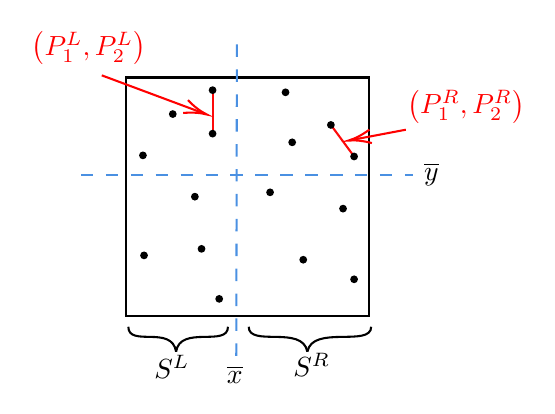
\begin{tikzpicture}[x=0.75pt,y=0.75pt,yscale=-1,xscale=1]
%uncomment if require: \path (0,325); %set diagram left start at 0, and has height of 325

%Shape: Rectangle [id:dp6499204868826074] 
\draw   (80.93,157.92) -- (198.12,157.92) -- (198.12,272.62) -- (80.93,272.62) -- cycle ;
%Straight Lines [id:da837478004805259] 
\draw [color={rgb, 255:red, 74; green, 144; blue, 226 }  ,draw opacity=1 ] [dash pattern={on 4.5pt off 4.5pt}]  (59.2,204.85) -- (219,204.85) ;
%Straight Lines [id:da7194776025159269] 
\draw [color={rgb, 255:red, 74; green, 144; blue, 226 }  ,draw opacity=1 ] [dash pattern={on 4.5pt off 4.5pt}]  (134.31,142) -- (134,295) ;


\draw [color={rgb, 255:red, 253; green, 10; blue, 10 }  ,draw opacity=1 ]   (122.59,164) -- (122.59,184.95) ;
%Straight Lines [id:da715666979908854] 
\draw [color={rgb, 255:red, 253; green, 10; blue, 10 }  ,draw opacity=1 ]   (179.58,180.76) -- (190.77,195.95) ;
%Straight Lines [id:da6970165255401948] 
\draw [color={rgb, 255:red, 255; green, 0; blue, 0 }  ,draw opacity=1 ]   (215.7,183.06) -- (189.96,187.93) ;
\draw [shift={(188,188.3)}, rotate = 349.29] [color={rgb, 255:red, 255; green, 0; blue, 0 }  ,draw opacity=1 ][line width=0.75]    (10.93,-3.29) .. controls (6.95,-1.4) and (3.31,-0.3) .. (0,0) .. controls (3.31,0.3) and (6.95,1.4) .. (10.93,3.29)   ;
%Straight Lines [id:da5840245566165858] 
\draw [color={rgb, 255:red, 255; green, 0; blue, 0 }  ,draw opacity=1 ]   (69.21,156.87) -- (117.94,175.03) ;
\draw [shift={(119.82,175.73)}, rotate = 200.44] [color={rgb, 255:red, 255; green, 0; blue, 0 }  ,draw opacity=1 ][line width=0.75]    (10.93,-3.29) .. controls (6.95,-1.4) and (3.31,-0.3) .. (0,0) .. controls (3.31,0.3) and (6.95,1.4) .. (10.93,3.29)   ;
%Shape: Free Drawing [id:dp8916770831600931] 
\filldraw (103.41,175.52) circle (1pt) ;
%Shape: Free Drawing [id:dp7205705113694219] 
\filldraw (179.58,180.76) circle (1pt);
%Shape: Free Drawing [id:dp5723003936317532] 
\filldraw (166.27,245.7) circle (1pt);
%Shape: Free Drawing [id:dp19778776200558257] 
\filldraw (89.56,243.61) circle (1pt);
%Shape: Free Drawing [id:dp22218199289458562] 
\filldraw (150.29,213.23) circle (1pt);
%Shape: Free Drawing [id:dp9270216931653172] 
\filldraw (157.74,165.04) circle (1pt);
%Shape: Free Drawing [id:dp30577755696643694] 
\filldraw (89.03,195.42) circle (1pt);
%Shape: Free Drawing [id:dp8352617777328899] 
\filldraw (125.78,264.56) circle (1pt);
%Shape: Free Drawing [id:dp007121195742592068] 
\filldraw (190.77,255.13) circle (1pt);
%Shape: Free Drawing [id:dp9787419741468635] 
\filldraw (160.94,189.14) circle (1pt);
%Shape: Free Drawing [id:dp05782734388952204] 
\filldraw (114.06,215.32) circle (1pt);
%Shape: Free Drawing [id:dp020809307556031387] 
\filldraw (122.59,184.95) circle (1pt);
%Shape: Free Drawing [id:dp9236450749534464] 
\filldraw (117.26,240.46) circle (1pt);
%Shape: Free Drawing [id:dp9814876804759312] 
\filldraw (185.44,221.08) circle (1pt);
%Shape: Free Drawing [id:dp32677091280799897] 
\filldraw (190.77,195.95) circle (1pt);
%Shape: Free Drawing [id:dp7375869135394859] 
\filldraw (122.59,164) circle (1pt) ;
%Straight Lines [id:da2008032684012] 
%Curve Lines [id:da7178341035011966] 
\draw    (82,278) .. controls (82,288) and (103,277) .. (105,290) ;
%Curve Lines [id:da31697667567298216] 
\draw    (130,278) .. controls (130,288) and (107,277) .. (105,290) ;
%Curve Lines [id:da6058144347191174] 
\draw    (140,278) .. controls (140,288) and (165.81,277) .. (168.27,290) ;
%Curve Lines [id:da842179996151678] 
\draw    (199,278) .. controls (199,288) and (170.73,277) .. (168.27,290) ;

% Text Node
\draw (223,197.4) node [anchor=north west][inner sep=0.75pt]    {$\overline{y}$};
% Text Node
\draw (128,295.4) node [anchor=north west][inner sep=0.75pt]    {$\overline{x}$};
% Text Node
\draw (215,162.4) node [anchor=north west][inner sep=0.75pt]  [color={rgb, 255:red, 255; green, 0; blue, 0 }  ,opacity=1 ]  {$\left( P_{1}^{R} ,P_{2}^{R}\right)$};
% Text Node
\draw (34,134.4) node [anchor=north west][inner sep=0.75pt]  [color={rgb, 255:red, 255; green, 0; blue, 0 }  ,opacity=1 ]  {$\left( P_{1}^{L} ,P_{2}^{L}\right)$};
% Text Node
\draw (93,290.4) node [anchor=north west][inner sep=0.75pt]    {$S^{L}$};
% Text Node
\draw (160,289.4) node [anchor=north west][inner sep=0.75pt]    {$S^{R}$};


\end{tikzpicture}


    \end{minipage}
\end{center}

\subsection{Conquer} Now we will recursively get pair of closest points in $S_L$ and $S_R$. Suppose the $(P_1^L,P_2^L)$ are the closest pair of points in $S^L$ and $(P_1^R,P_2^R)$ are the closest pair of points in $S^R$.

\begin{algorithm}[H]
        \DontPrintSemicolon
            \SetKwProg{Fn}{Function}{:}{}
            \Fn{Conquer}{
                Solve for $S_L,S^R$.\;
                $(P_1^L,P_2^L)$ are closest pair of points in $S_L$.\;
                $(P_1^R,P_2^R)$ are closest pair of points in $S_R$.\;
                $\delta^L=d(P_1^L,P_2^L)$, $\delta^R=d(P_1^R,P_2^R)$\;
                $\delta_{min}\longleftarrow \min \{\delta^L,\delta^R\}$
            }
            \caption{Step 1 (Solve Subproblems)}
        \end{algorithm}

\subsection{Combine}     Now we want to combine these two solutions. 
\begin{question}{We are not done}{}
Is there a pair of points $P_i,P_j\in S$ such that $d(P_i,P_j)<\delta_{min}$
\end{question}
If Yes: \begin{itemize}
\item One of them must be in $S_L$ and the other is in $S_R$. 
\item $x-$coordinate $\in [\ovx-\delta_{min},\ovx+\delta_{min}]$. 
\item $|y_i-y_j|\leq \delta_{min}$
\end{itemize}
\parinf 

So we take the strip of radius $\delta_{min}$ around $\ovx$. Define $T=\{P_i\in S\mid |x_i-\ovx|\leq \delta_{min}\}$

\begin{center}
       
    \tikzset{every picture/.style={line width=0.75pt}} %set default line width to 0.75pt        

    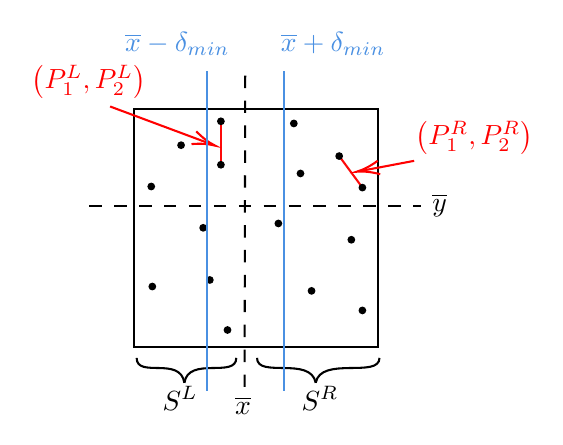
\begin{tikzpicture}[x=0.75pt,y=0.75pt,yscale=-1,xscale=1]
    %uncomment if require: \path (0,325); %set diagram left start at 0, and has height of 325
    
    %Shape: Rectangle [id:dp6499204868826074] 
    \draw   (80.93,157.92) -- (198.12,157.92) -- (198.12,272.62) -- (80.93,272.62) -- cycle ;
    %Straight Lines [id:da837478004805259] 
    \draw [color={rgb, 255:red, 0; green, 0; blue, 0 }  ,draw opacity=1 ] [dash pattern={on 4.5pt off 4.5pt}]  (59.2,204.85) -- (219,204.85) ;
    %Straight Lines [id:da7194776025159269] 
    \draw [color={rgb, 255:red, 0; green, 0; blue, 0 }  ,draw opacity=1 ] [dash pattern={on 4.5pt off 4.5pt}]  (134.31,142) -- (134,295) ;
    %Straight Lines [id:da2008032684012] 
    \draw [color={rgb, 255:red, 253; green, 10; blue, 10 }  ,draw opacity=1 ]   (122.59,164) -- (122.59,184.95) ;
    %Straight Lines [id:da715666979908854] 
    \draw [color={rgb, 255:red, 253; green, 10; blue, 10 }  ,draw opacity=1 ]   (179.58,180.76) -- (190.77,195.95) ;
    %Straight Lines [id:da6970165255401948] 
    \draw [color={rgb, 255:red, 255; green, 0; blue, 0 }  ,draw opacity=1 ]   (215.7,183.06) -- (189.96,187.93) ;
    \draw [shift={(188,188.3)}, rotate = 349.29] [color={rgb, 255:red, 255; green, 0; blue, 0 }  ,draw opacity=1 ][line width=0.75]    (10.93,-3.29) .. controls (6.95,-1.4) and (3.31,-0.3) .. (0,0) .. controls (3.31,0.3) and (6.95,1.4) .. (10.93,3.29)   ;
    %Straight Lines [id:da5840245566165858] 
    \draw [color={rgb, 255:red, 255; green, 0; blue, 0 }  ,draw opacity=1 ]   (69.21,156.87) -- (117.94,175.03) ;
    \draw [shift={(119.82,175.73)}, rotate = 200.44] [color={rgb, 255:red, 255; green, 0; blue, 0 }  ,draw opacity=1 ][line width=0.75]    (10.93,-3.29) .. controls (6.95,-1.4) and (3.31,-0.3) .. (0,0) .. controls (3.31,0.3) and (6.95,1.4) .. (10.93,3.29)   ;
    %Shape: Free Drawing [id:dp8916770831600931] 
    \filldraw (103.41,175.52) circle (1pt);
    %Shape: Free Drawing [id:dp7205705113694219] 
    \filldraw (179.58,180.76) circle (1pt);
    %Shape: Free Drawing [id:dp5723003936317532] 
    \filldraw (166.27,245.7) circle (1pt);
    %Shape: Free Drawing [id:dp19778776200558257] 
    \filldraw (89.56,243.61) circle (1pt);
    %Shape: Free Drawing [id:dp22218199289458562] 
    \filldraw (150.29,213.23) circle (1pt);
    %Shape: Free Drawing [id:dp9270216931653172] 
    \filldraw (157.74,165.04) circle (1pt);
    %Shape: Free Drawing [id:dp30577755696643694] 
    \filldraw (89.03,195.42) circle (1pt);
    %Shape: Free Drawing [id:dp8352617777328899] 
    \filldraw (125.78,264.56) circle (1pt);
    %Shape: Free Drawing [id:dp007121195742592068] 
    \filldraw (190.77,255.13) circle (1pt);
    %Shape: Free Drawing [id:dp9787419741468635] 
    \filldraw (160.94,189.14) circle (1pt);
    %Shape: Free Drawing [id:dp05782734388952204] 
    \filldraw (114.06,215.32) circle (1pt);
    %Shape: Free Drawing [id:dp020809307556031387] 
    \filldraw (122.59,184.95) circle (1pt);
    %Shape: Free Drawing [id:dp9236450749534464] 
    \filldraw (117.26,240.46) circle (1pt);
    %Shape: Free Drawing [id:dp9814876804759312] 
    \filldraw (185.44,221.08) circle (1pt);
    %Shape: Free Drawing [id:dp32677091280799897] 
    \filldraw (190.77,195.95) circle (1pt);
    %Shape: Free Drawing [id:dp7375869135394859] 
    \filldraw (122.59,164) circle (1pt);
    %Curve Lines [id:da7178341035011966] 
    \draw    (82,278) .. controls (82,288) and (103,277) .. (105,290) ;
    %Curve Lines [id:da31697667567298216] 
    \draw    (130,278) .. controls (130,288) and (107,277) .. (105,290) ;
    %Curve Lines [id:da6058144347191174] 
    \draw    (140,278) .. controls (140,288) and (165.81,277) .. (168.27,290) ;
    %Curve Lines [id:da842179996151678] 
    \draw    (199,278) .. controls (199,288) and (170.73,277) .. (168.27,290) ;
    %Straight Lines [id:da01763770038587964] 
    \draw [color={rgb, 255:red, 74; green, 144; blue, 226 }  ,draw opacity=1 ]   (153,140) -- (153,294) ;
    %Straight Lines [id:da6702110585391772] 
    \draw [color={rgb, 255:red, 74; green, 144; blue, 226 }  ,draw opacity=1 ]   (116,140) -- (116,294) ;
    
    % Text Node
    \draw (223,197.4) node [anchor=north west][inner sep=0.75pt]    {$\overline{y}$};
    % Text Node
    \draw (128,295.4) node [anchor=north west][inner sep=0.75pt]    {$\overline{x}$};
    % Text Node
    \draw (215,162.4) node [anchor=north west][inner sep=0.75pt]  [color={rgb, 255:red, 255; green, 0; blue, 0 }  ,opacity=1 ]  {$\left( P_{1}^{R} ,P_{2}^{R}\right)$};
    % Text Node
    \draw (30,135.4) node [anchor=north west][inner sep=0.75pt]  [color={rgb, 255:red, 255; green, 0; blue, 0 }  ,opacity=1 ]  {$\left( P_{1}^{L} ,P_{2}^{L}\right)$};
    % Text Node
    \draw (93,290.4) node [anchor=north west][inner sep=0.75pt]    {$S^{L}$};
    % Text Node
    \draw (160,290.4) node [anchor=north west][inner sep=0.75pt]    {$S^{R}$};
    % Text Node
    \draw (150,119.4) node [anchor=north west][inner sep=0.75pt]  [color={rgb, 255:red, 74; green, 144; blue, 226 }  ,opacity=1 ]  {$\overline{x} +\delta _{min}$};
    % Text Node
    \draw (75,119.4) node [anchor=north west][inner sep=0.75pt]  [color={rgb, 255:red, 74; green, 144; blue, 226 }  ,opacity=1 ]  {$\overline{x} -\delta _{min}$};
    
    
    \end{tikzpicture}
\end{center}
We now sort all the points in the $T$ by their decreasing $y-$coordinate. Let $T_y$ be the array of points. For each $P_i\in T_y$ define the region $$T_i=\{P_j\in T_y \mid 0\leq y_j-y_i\leq \delta_{min}, j>i\}$$

\pagebreak
\begin{center}
	\begin{minipage}{0.7\textwidth}

\begin{lemma}{}{}
	Number of points (other than $P_i$) that lie inside the box is at most 8
\end{lemma}
\begin{proof}
	Suppose there are more than 8 points that lie inside the box apart from $P_i$. The box has a left square part and a right square part. So one of the squares contains at least 5 points. WLOG suppose the left square has at least 5 points. Divide each square into 4 parts by a middle vertical and a middle horizontal line. Now since there are 5 points there is one part which contains 2 points but that is not possible as those two points are in $S_L$ and their distance will be less than $\delta_{min}$ which is not possible. Hence contradiction. Therefore there are at most 8 points inside the box.
\end{proof}\parinn

Hence by the above lemma for each $P_i\in T_y$ there are at most 8 points in $T_i$. So for each $P_j\in T_i$ we find the $d(P_i,P_j)$ and if it is less than $\delta_{min}$ we update the points and the distance
	\end{minipage}
\hspace{1cm}
\begin{minipage}{0.229\textwidth}
	


\tikzset{every picture/.style={line width=0.75pt}} %set default line width to 0.75pt        

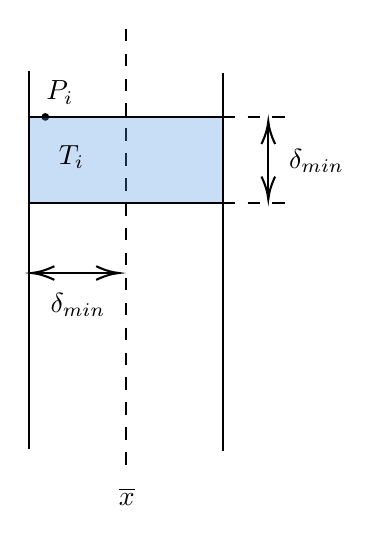
\begin{tikzpicture}[x=0.75pt,y=0.75pt,yscale=-1,xscale=1]
	%uncomment if require: \path (0,300); %set diagram left start at 0, and has height of 300
	
	%Straight Lines [id:da3975720681427135] 
	\draw    (200,50.92) -- (200,233.14) ;
	%Straight Lines [id:da42362227502058447] 
	\draw    (293.43,51.98) -- (293.43,234.2) ;
	%Straight Lines [id:da04130491026490812] 
	\draw  [dash pattern={on 4.5pt off 4.5pt}]  (246.71,30.67) -- (246.71,244.38) ;
	%Straight Lines [id:da4384742510539741] 
	\draw    (200,73.3) -- (293.43,73.3) ;
	%Straight Lines [id:da3745552754160917] 
	\draw    (200,114.85) -- (293.43,114.85) ;
	%Straight Lines [id:da9873374520652576] 
	\draw    (203.43,148.38) -- (241.43,148.38) ;
	\draw [shift={(243.43,148.38)}, rotate = 180] [color={rgb, 255:red, 0; green, 0; blue, 0 }  ][line width=0.75]    (10.93,-3.29) .. controls (6.95,-1.4) and (3.31,-0.3) .. (0,0) .. controls (3.31,0.3) and (6.95,1.4) .. (10.93,3.29)   ;
	\draw [shift={(201.43,148.38)}, rotate = 0] [color={rgb, 255:red, 0; green, 0; blue, 0 }  ][line width=0.75]    (10.93,-3.29) .. controls (6.95,-1.4) and (3.31,-0.3) .. (0,0) .. controls (3.31,0.3) and (6.95,1.4) .. (10.93,3.29)   ;
	%Straight Lines [id:da5826410245797784] 
	\draw    (315.43,77.3) -- (315.43,110.85) ;
	\draw [shift={(315.43,112.85)}, rotate = 270] [color={rgb, 255:red, 0; green, 0; blue, 0 }  ][line width=0.75]    (10.93,-3.29) .. controls (6.95,-1.4) and (3.31,-0.3) .. (0,0) .. controls (3.31,0.3) and (6.95,1.4) .. (10.93,3.29)   ;
	\draw [shift={(315.43,75.3)}, rotate = 90] [color={rgb, 255:red, 0; green, 0; blue, 0 }  ][line width=0.75]    (10.93,-3.29) .. controls (6.95,-1.4) and (3.31,-0.3) .. (0,0) .. controls (3.31,0.3) and (6.95,1.4) .. (10.93,3.29)   ;
	%Straight Lines [id:da8728720299963784] 
	\draw  [dash pattern={on 4.5pt off 4.5pt}]  (293.43,73.3) -- (329.43,73.3) ;
	%Straight Lines [id:da06933695064552192] 
	\draw  [dash pattern={on 4.5pt off 4.5pt}]  (293.43,114.85) -- (324.43,114.85) ;
	%Shape: Free Drawing [id:dp435305414025839] 
	\filldraw (208,73.17) circle (1pt) ;
	%Shape: Rectangle [id:dp914080675609527] 
	\draw  [fill={rgb, 255:red, 74; green, 144; blue, 226 }  ,fill opacity=0.3 ] (200,73.3) -- (293.43,73.3) -- (293.43,114.85) -- (200,114.85) -- cycle ;
	
	% Text Node
	\draw (209,156.4) node [anchor=north west][inner sep=0.75pt]    {$\delta _{min}$};
	% Text Node
	\draw (324,87.4) node [anchor=north west][inner sep=0.75pt]    {$\delta _{min}$};
	% Text Node
	\draw (207,54.4) node [anchor=north west][inner sep=0.75pt]    {$P_{i}$};
	% Text Node
	\draw (242,250.4) node [anchor=north west][inner sep=0.75pt]    {$\overline{x}$};
	% Text Node
	\draw (213,85.4) node [anchor=north west][inner sep=0.75pt]    {$T_{i}$};
	
	
\end{tikzpicture}
\end{minipage}
\end{center}
\subsection{Pseudocode and Time Complexity}
\begin{assumption*}
	We will assume for now that for all $P_i.P_j\in S$ we have $x_i\neq x_j$ and $y_i\neq y_j$. Later we will modify the pseudocode to remove this assumption
\end{assumption*}
\begin{algorithm}
	\DontPrintSemicolon
	\KwIn{Set of $n$ points, $S=\{(x_i,y_i)\mid x_i,y_i\in\bbR, \ \forall\ i\in[n]\}$. We denote $P_i=(x_i,y_i)$. }
	\KwOut{Closest pair of ponts, $(P_i,P_j,\delta)$ where $\delta=d(P_i,P_j)$}
	\Begin{
\If{$|S|\leq 10$}{Solve by Brute Force (Consider every pair of points)}	

$S^x\longleftarrow S$ sorted by $x-$coordinate, \hspace{5mm} $S^y\longleftarrow S$ sorted by $y-$coordinate\;
$\ovx\longleftarrow \lfloor \frac{n}{2}\rfloor $ highest $x-$coordinate, \hspace{5mm} $\ovy\longleftarrow \lfloor \frac{n}{2}\rfloor $ highest $y-$coordinate\;
$S^L\longleftarrow \{P_i\mid x_i<\bar{x},\ \forall\ i\in[n]\}$, \hspace{5mm} $S^R\longleftarrow \{P_i\mid x_i\geq\bar{x},\ \forall\ i\in[n]\}$\;
$(P_1^L,P_2^L,\delta^L)\longleftarrow$ \textsc{Find-Closest}($S^L$), \hspace{5mm} $(P_1^R,P_2^R,\delta^R)\longleftarrow$ \textsc{Find-Closest}($S^R$)\;
$\delta_{min}\longleftarrow \min\{\delta^L,\delta^R\}$\;
\If{$\delta_{min}<\delta^L$}{$P_1\longleftarrow P_1^R$, $P_2\longleftarrow P_2^R$}

\Else{$P_1\longleftarrow P_1^L$, $P_2\longleftarrow P_2^L$}
$T\longleftarrow \{P_i\mid |x_i-\ovx|\leq \delta_{min}\}$\;
$T_y\longleftarrow T$ sorted by decreasing $y-$coordinate\;
\For{$P\in T_y$}{
$U\longleftarrow $ Next $8$ points\;
\For{$\hat{P}\in U$}{
\If{$d(P,\hat{P})<\delta_{min}$}{$\delta_{min}\longleftarrow d(P,\hat{P})$\;
$(P_1,P_2)\longleftarrow (P,\hat{P})$}
}
}
\Return{$(P_1,P_2,\delta_{min})$}
}

	\caption{\textsc{Find-Closest}($S$)}
	\label{find-closest-nlog2n}	
\end{algorithm}

Notice we used the assumption in the line $5$ for finding the medians. So the line 4 takes $O(n\log n)$ times. Lines 5,6 takes $O(n)$ time. Since $\ovx$ is the median, we have  $|S^L|=\lfloor \frac{n}2\rfloor$ and $|S^R|=\lceil \frac{n}{2}\rceil$. Hence $\textsc{Find-Closest}(S^L)$ and $\textsc{Find-Closest}(S^R)$ takes $T\lt(\frac{n}{2}\rt)$ time. Now lines $8-12$ takes constant time. Line 13 takes $O(n)$ time. And line 14 takes $O(n\log n)$ time. Since $U$ has 8 points i.e. constant number of points the lines $16-20$ takes constant time for each $P\in T_y$. Hence the for loop at line 15 takes $O(n)$ time. Hence total time taken $$T(n)=O(n)+O(n\log n)+2T\lt(\frac{n}2\rt)\implies T(n)=O(n\log^2n)$$
\section{Improved Algorithm for $O(n\log n)$ Runtime}
Notice once we sort the points by $x-$coordinate and $y-$coordinate we don't need to sort the points anymore. We can just pass the sorted array of points into the arguments for solving the smaller problems. Their is another time where we need to sort which is in line 14 of the above algorithm. This we can get actually from $S^y$ without sorting just checking one by one backwards direction if the $x-$coordinate of the points satisfy $|x_i-\ovx|\leq \delta_{min}$. So $$T_y=\textsc{Reverse}(\{P_i\in S^y\mid |x_i-\ovx|\leq \delta_{min}\})$$

So we form a new algorithm which takes the input $S^x$ and $S^y$ and then finds the closest pair of points. Then we will use that subroutine to find closest pair of points in any given set of points.

\begin{center}
	\begin{minipage}{0.55\textwidth}
\begin{algorithm}[H]
	\DontPrintSemicolon
	\KwIn{Set of $n$ points, $S=\{(x_i,y_i)\mid x_i,y_i\in\bbR, \ \forall\ i\in[n]\}$.		
		$S^x$ and $S^y$ are the sorted  array of points with respect to $x-$coordinate and $y-$coordinate respectively}
	\KwOut{Closest pair of ponts, $(P_i,P_j,\delta)$ where $\delta=d(P_i,P_j)$}
	\Begin{
		\If{$|S|\leq 10$}{Solve by Brute Force}	
		
		$\ovx\longleftarrow \lfloor \frac{n}{2}\rfloor $ highest $x-$coordinate\;
		  $\ovy\longleftarrow \lfloor \frac{n}{2}\rfloor $ highest $y-$coordinate\;
		$S^L\longleftarrow \{P_i\in S^x\mid x_i<\bar{x},\ \forall\ i\in[n]\}$\;
		$S^L_y\longleftarrow \{P_i\in S^y\mid x_i<\ovx\}$\;
		  $S^R\longleftarrow \{P_i\in S^x\mid x_i\geq\bar{x},\ \forall\ i\in[n]\}$\;
		  $S^R_y\longleftarrow \{P_i\in S^y\mid x_i\geq \ovx\}$\;
		$(P_1^L,P_2^L,\delta^L)\longleftarrow$ \textsc{Find-Closest-Sorted}($S^L,S^L_y$)\;
		  $(P_1^R,P_2^R,\delta^R)\longleftarrow$ \textsc{Find-Closest-Sorted}($S^R,S^R_y$)\;
		$\delta_{min}\longleftarrow \min\{\delta^L,\delta^R\}$\;
		\If{$\delta_{min}<\delta^L$}{$P_1\longleftarrow P_1^R$, $P_2\longleftarrow P_2^R$}
		
		\Else{$P_1\longleftarrow P_1^L$, $P_2\longleftarrow P_2^L$}
		$T\longleftarrow \{P_i\mid |x_i-\ovx|\leq \delta_{min}\}$\;
		$T_y\longleftarrow \textsc{Reverse}(\{P_i\in S^y\mid |x_i-\ovx|\leq \delta_{min}\})$\;
		\For{$P\in T_y$}{
			$U\longleftarrow $ Next $8$ points\;
			\For{$\hat{P}\in U$}{
				\If{$d(P,\hat{P})<\delta_{min}$}{$\delta_{min}\longleftarrow d(P,\hat{P})$\;
					$(P_1,P_2)\longleftarrow (P,\hat{P})$}
			}
		}
		\Return{$(P_1,P_2,\delta_{min})$}
	}
	
	\caption{\textsc{Find-Closest-Sorted}($S^x,S^y$)}
	\label{find-closest-nlog2n}	
\end{algorithm}
	\end{minipage}
\hspace{0.1mm}
	\begin{minipage}{0.43\textwidth}
\begin{algorithm}[H]
	\DontPrintSemicolon
	\KwIn{Set of $n$ points, $S=\{(x_i,y_i)\mid x_i,y_i\in\bbR, \ \forall\ i\in[n]\}$. We denote $P_i=(x_i,y_i)$. }
	\KwOut{Closest pair of ponts, $(P_i,P_j,\delta)$ where $\delta=d(P_i,P_j)$}
	\Begin{
		\If{$|S|\leq 10$}{Solve by Brute Force}	
	$S^x\longleftarrow S$ sorted by $x-$coordinate\;
	 $S^y\longleftarrow S$ sorted by $y-$coordinate\;
	 \Return{\textsc{Find-Closest-Sorted}$(S^x,S^y)$}
}
	\caption{\textsc{Find-Closest}($S$)}
\end{algorithm}
\end{minipage}
\end{center}


This algorithm only sorts one time. So time complexity for $\textsc{Find-Closest-Sorted}(S^x,S^y)$ is $$T(n)=2T\lt(\frac{n}{2}\rt)+O(n)\implies T(n)=O(n\log n)$$and therefore times complexity for $\textsc{Find-Closest}(S)$ is $O(n\log n)$. 

\section{Removing the Assumption}
For this there nothing much to do. For finding the median $\ovx$ if we have more than one points with same $x-$coordinate which appears as the $\lt\lfloor \frac{n}{2}\rt\rfloor$ highest $x-$coordinate we sort only those points with respect to their $y-$coordinate update the $S^x$ like that and then take $\lt\lfloor \frac{n}{2}\rt\rfloor$ highest point in $S^x$. We do the same for $S^y$ and update accordingly. All this we do so that $S^L$ and $S^R$ has the size $\frac{n}{2}$. 
